\documentclass[11pt,a4paper]{article}

% -------------------------------------------------
% Packages
% -------------------------------------------------
\usepackage{geometry}
\geometry{margin=2.5cm}
\usepackage{newpxtext}
\usepackage{amsmath, amssymb, bm}
\usepackage{graphicx}
\usepackage{hyperref}
\usepackage{physics}
\usepackage{enumitem}
\usepackage{caption}
\usepackage{booktabs}
\usepackage[
  backend=bibtex,
  style=authoryear,
  sorting=none
]{biblatex}
\usepackage{caption}
\addbibresource{bibliography.bib}
% -------------------------------------------------
% Title
% -------------------------------------------------
\title{\textbf{StonedFenicsx}\\
\large Kinematic thermal numerical code for slab temperature evolution}

\author{Andrea Piccolo, Tim Craig, Iris Van Zelst, Cedric Thileoult}
\date{12.12.2025}

\begin{document}
\maketitle

\begin{center}
  \includegraphics[width=1.0\textwidth]{Temp_Slab.png}
\end{center}

\vspace{1em}

% =================================================
\section*{Introduction}
% =================================================

%Presentation
StonedFenicsx is a kinematic thermal numerical code designed to describe the
thermal evolution of subducting slabs using the Finite Element Method (FEM). The main purpose of the code is to assess the impact of non-linear thermal properties on the evolution of a kinematically driven subduction. 

% The importance of temperature evolution for understanding present-day subduction zone.
To study the present-day subduction zone, it is necessary to have a means to accurately estimate the subducting plate thermal structure. The thermal structure of the subducting plate exerts a first-order control on the subduction processes. During the descendant of a subducting plate, the rocks heat and undergo metamorphic processes. The metamorphic reactions involving the hydrated minerals release fluids. Fluids can alter the frictional stability of the  materials by perturbing the stress and pressure field through the increase of in pore-fluid pressure. Moreover, fluids can escape from the source area and can percolate upward metasomatizing the mantle. The latter process leads to the decompression of the mantle's solidus, causing partial melting and consequent arc volcanism. Knowing the thermal structure of the subducting plate is important for predicting the potential hazards in a subduction zone \parencite{hobson2025sensitivity}. Moreover, since many geophysical signals depend on material properties that depend on temperature and composition, having an accurate estimation of the thermal structure of the slab improves the interpretation of the geophysical data.

%How to study subduction zone 
Subduction dynamics can be studied using full dynamical model or imposing a kinematically driven flow \parencite{van2023introductory,holt2021slab}. To understand the physical mechanisms behind the subduction processes, it is necessary to describe and model the temporal evolution of the subduction. Dynamical model, in this case, are the right choice, because they allow to describe how the stress, strain-rate evolves with time as a consequence of the time-dependent evolution of the system. But, due to the numerous parameters that controls the resulting geometry and final thermal structure of the descending plate, dynamic models are too computationally expensive for studying specific subduction zones and relative geophysical data-set. Kinematical models, in this latter case, are extremely useful, because it is possible to define the velocity field and the geometry of the target subduction zone and exploring what parameters best fit the current observations. 

%Kinematical model 
Kinematical models are often used for understanding the present-day temperature field. The present-day temperature field within the subduction zone and mantle wedge, can be used to constraint and interpret the geophysical observations. The combination of the results of such modelling with petrological forward modelling allow to interpret the intermediate seismicity, and potential loci of fluid generation. Most of the kinematic models rely on simple assumptions: 1st that the steady state solution for a given velocity field is representative of the present-day temperature field; 2nd that the thermal properties are not changing as a function of pressure and temperature. There have been a few attempts to explore the effects of non-linear thermal properties, however, either were not applied to specific subduction zone, or they were designed to explore the implication on the whole subduction system. StonedFenicsx has been developed to verify whether or not the consideration of such linearities improve the interpretation of the geophysical data of present-day specific subduction zone. 

% What are the main idea of the code

The temperature evolution depends on the initial state of the system (i.e., the age of the plate), frictional heating at the interface between the subducting and overriding plates, and mantle-wedge flow. The resulting thermal field depends on the heat capacity, thermal conductivity, and density of the material. These material properties vary as a function of mineralogical composition, pressure, and temperature. The purpose of Stonedfenicsx is to test the effects of compositional and thermal non-linearities on the thermal evolution of kinematically driven subduction models. The numerical framework is capable of handling the non-linearities associated with thermal properties and accounts, in a simplified but consistent manner, for adiabatic transformations. In a second stage, forward petrological modelling will be incorporated to assess the impact of mineralogical changes on the final thermal state. The fundamental question is whether these additional complexities improve the interpretation of existing datasets.
% =================================================
\section*{Methods}
% =================================================

\subsection*{Equations}

StonedFenicsx solves the continuity, momentum, and energy conservation equations
using FEM. The numerical model is fully driven by kinematic boundary conditions.
The medium is incompressible and the momentum equation does not include
gravitational body forces.

\paragraph{Mass conservation}
\begin{equation}
\nabla \cdot \mathbf{u} = 0
\end{equation} \label{eq:mass_conversation}
where $\mathbf{u}$ is the velocity field.

\paragraph{Momentum conservation}
\begin{equation}
\nabla \cdot \bm{\tau} + \nabla P = 0
\end{equation}\label{eq:momentum_equation}

The deviatoric stress tensor is defined as
\begin{equation}
\bm{\tau} = 2 \, \eta_{\mathrm{eff}} \, \dot{\bm{\varepsilon}}
\end{equation}\label{eq:deviatoric_stress}

with the deviatoric strain-rate tensor
\begin{equation}
\dot{\bm{\varepsilon}} =
\frac{1}{2}\left( \nabla \mathbf{u} + \nabla \mathbf{u}^{T} \right)
\end{equation}\label{eq:strain_rate_tensor}

The second invariant of the strain rate is
\begin{equation}
\dot{\varepsilon}_{II} =
\sqrt{\frac{1}{2}\, \dot{\bm{\varepsilon}} : \dot{\bm{\varepsilon}}}
\end{equation}\label{eq:strain_rate_invariant}

The effective viscosity depends on temperature, pressure, and strain rate:
\begin{equation}
\eta_{\mathrm{eff}} = f(T,P,\dot{\varepsilon}_{II})
\end{equation}\label{eq:viscosity}

% -------------------------------------------------
\subsection*{Energy Conservation}
% -------------------------------------------------

\paragraph{Steady state}
\begin{equation}
\nabla \cdot (k \nabla T) + \rho C_p \nabla \cdot T + H = 0
\end{equation}

\paragraph{Time dependent}
\begin{equation}
\rho C_p \frac{\partial T}{\partial t}
+ \rho C_p \nabla \cdot T
+ \nabla \cdot (k \nabla T)
+ H = 0
\end{equation}

where:
\begin{itemize}[leftmargin=*]
\item $k$ is thermal conductivity [$\mathrm{W\,m^{-1}\,K^{-1}}$]
\item $C_p$ is heat capacity [$\mathrm{J\,kg^{-1}\,K^{-1}}$]
\item $\rho$ is density [$\mathrm{kg\,m^{-3}}$]
\item $H$ is the volumetric heat source (shear, radiogenic and adiabatic heating) [$\mathrm{W\,m^{-3}}$]
\end{itemize}

% -------------------------------------------------
\subsection*{Lithostatic Pressure}
% -------------------------------------------------

Material properties depend on pressure and temperature. Since dynamic pressure
computed without gravity is unreliable, a lithostatic pressure field is computed
following \parencite{jourdon2022efficient}.

\begin{equation}
\nabla \cdot \nabla P^{L} - \nabla \cdot (\rho \mathbf{g}) = 0
\end{equation}

This lithostatic pressure field is used to evaluate material properties as a
function of depth. Moreover, it is used for computing the adiabatic contribution. 

% =================================================
\section*{Numerical Methods}
% =================================================

The equations are discretised using FEM. Assembly and discretisation are handled
by the \texttt{dolfinx}, \texttt{ufl}, and \texttt{basix} libraries \parencite{baratta2023dolfinx,alnaes2014unified,scroggs2022construction,scroggs2022basix}.


% =================================================
\section*{Material Properties}
% =================================================

\subsection*{Rheology}

The effective viscosity is defined as
\begin{equation}
\eta =
\frac{1}{2} B^{-1/n} d^{-m}
\dot{\varepsilon}_{II}^{\frac{1-n}{n}}
\exp\!\left( \frac{E + PV}{nRT} \right)
\end{equation}

The effective viscosity is computed as a harmonic average:
\begin{equation}
\eta_{\mathrm{eff}} =
\left(
\frac{1}{\eta_{\mathrm{dif}}}
+ \frac{1}{\eta_{\mathrm{dis}}}
+ \frac{1}{\eta_{\max}}
\right)^{-1}
\end{equation}

% -------------------------------------------------
\subsection*{Density}
% -------------------------------------------------

\begin{equation}
\rho = \rho_0 \exp(cf_T)\exp(cf_P)
\end{equation}

with
\begin{align}
cf_T &= \alpha_0 (T-T_0) + \frac{\alpha_1}{2}(T^2 - T_0^2) \\
cf_P &= \beta P
\end{align}

% -------------------------------------------------
\subsection*{Heat Capacity}
% -------------------------------------------------

\begin{equation}
C_p =
C_{p0}
+ C_{p1}T^{-0.5}
+ C_{p2}T^{-2}
+ C_{p3}T^{-3}
+ C_{p4}T
+ C_{p5}T^2
\end{equation}

% -------------------------------------------------
\subsection*{Thermal Conductivity}
% -------------------------------------------------

\begin{center}
  \includegraphics[width=0.8\textwidth]{thermal_conductivity_total.png}
\end{center}

\begin{equation}
k(P,T) =
k_0 o_0
+ \kappa(T)\rho C_p
+ k_{\mathrm{rad}}(T)
\end{equation}

\begin{equation}
\kappa(T) =
\kappa_0
+ \kappa_1 e^{-\frac{T-T_0}{\kappa_2}}
+ \kappa_3 e^{-\frac{T-T_0}{\kappa_4}}
\end{equation}





% =================================================
\section*{Initial Setup and Boundary Conditions}
% =================================================

\begin{figure}[htbp]
  \centering
  \includegraphics[width=0.8\textwidth]{Initial_setup.png}
  \caption{\textbf{Simplified initial setup.} Simplified sketch of the numerical domain. The figure is based on the benchmark of \parencite{van2023introductory,van2008community}.}
  \label{fig:f1_simplified_initial_setup}
\end{figure}

The computational domain is generated using \texttt{gmsh} and consists of an unstructured triangular mesh \parencite{geuzaine2009gmsh}. In \textbf{Fig.}~\ref{fig:f1_simplified_initial_setup}, we sketch a simplified initial computational domain. In this sketch, we highlight the features that are common to all numerical realisations. The main portions of the numerical domain are shown using different colours, the points defining the physical boundaries are labelled with capital letters (\texttt{A–L}), and the boundaries are denoted by bracketed lowercase letters (\textbf{[a–i]}).

The main computational domain can be approximated by a trapezoid defined by \texttt{A}, \texttt{B}, \texttt{C}, \texttt{D}, \texttt{E} and \texttt{F}. The computational domain extends from the surface $0$ [km] to a maximum depth of $-600$ [km]. The horizontal extent of the numerical domain (\textit{i.e.,} the coordinate $x$ of \texttt{F} and \texttt{E}) depends on the geometry of the slab. The point \textbf{A} represents the origin, and it has coordinates $(0,0)$ [km]. The point \texttt{B} represents the base of the subducting plate and it is located at  $(0,-140)$ [km]. The points \texttt{C} and \texttt{D} have coordinates $(x_b,-600)$ [km] and $(x_t,-600)$ [km]; $x_b$ and $x_t$ values depend on the chosen geometry of the slab. \texttt{E} and \texttt{F} are the rightmost points and have coordinates $(x_t+60,-600)$ and  $(x_t+60,0)$ [km], respectively. 

 The initial setup is divided into three subdomains: \texttt{Slab} (\textbf{S}), \texttt{Wedge} (\textbf{W}) and 
\texttt{Overriding plate} (\textbf{OP}), coloured in red, yellow and grey, respectively. The subdivision is generated by two internal boundaries: the top surface of the slab, and the overriding plate boundary, line \texttt{[a]} and \texttt{[b]} in \textbf{Fig.} \ref{fig:f1_simplified_initial_setup}. The top surface of the slab (\texttt{[a]}) represents the kinematic boundary condition that drives the velocity field of the entire numerical domain. The velocity is imposed parallel to the top surface of the slab, and its magnitude is equal to the input convergence velocity. The base of \textbf{OP} is treated as a no-slip boundary condition.

The subdivision into three smaller domains is useful to simplify the computation of the Stokes equations: mass and momentum conservation are computed only in the \textbf{S} and \textbf{W} domains. Lithostatic pressure and energy conservation equations are solved in the entire domain. We will describe the main features of each subdomain in the following paragraphs. The subdomains represent indipendent and not overlapping computational domains. They are defined by specific boundaries, that are shared with other computational subdomains. Each subdomains can be composed by different material properties: for example, the overriding plate can be composed of crustal units and lithospheric mantle. The different material phases affect mostly the thermal properties. We described briefly the subdomains in which the Stokes equations are solved (slab and wedge) and the relative boundary conditions. After that, we will discuss the thermal boundary conditions that are applied for the global domain (\textbf{G} = \textbf{OP} +\textbf{S} +\textbf{W} ).

\subsection*{Slab}

In \textbf{Fig.} \ref{fig:f1_simplified_initial_setup}, \textbf{S} is shown in red, and it is defined by points \texttt{A}, \texttt{B}, \texttt{C} and \texttt{D}. It is bounded by four boundaries: \texttt{[a]},\texttt{[c]},\texttt{[d]} and \texttt{[e]}. On \texttt{[a]}, we prescribe an internal moving-wall boundary condition. The velocity $v_c$ represents the convergence velocity, and it is locally parallel to the tangent of \texttt{[a]}. The velocity vector is prescribed such that its magnitude is constant and equal to $v_c$. The boundary \texttt{[c]} is the base of the plate and we apply a free-slip boundary condition using the Nitsche method \parencite{sime2020automatic,sime2024thermal}. The boundaries \texttt{[d]} and \texttt{[e]} are open boundaries, whose inflow or outflow velocities depend on the magnitude of the convergence velocity applied to \texttt{[a]}. 

To optimise the computational cost, the viscosity within \textbf{S} is constant and equal to $\eta_{\mathrm{slab}}$, regardless the amount of the number of material phases within \textbf{S}. This allows us to solve the Stokes equations only once per numerical realisation, both for the steady-state and time-dependent problem. \textbf{S} can have different material phases: lithospheric mantle and oceanic crust. Each of these materials can have different heat capacity, density and conductivity. 

\subsection*{Wedge}

The \textbf{W} subdomain is defined by points \texttt{H}, \texttt{D}, \texttt{E} and \texttt{F} (see \textbf{Fig.}~\ref{fig:f1_simplified_initial_setup}). It is bounded by a portion of the boundary \texttt{[a]} (from point \texttt{H} to \texttt{D}), by the boundaries \texttt{[f]}, \texttt{[g]} and \texttt{[b]}. 

The boundaries \texttt{[f]} and \texttt{[g]} are open (do-nothing boundary conditions). \texttt{[f]} is mostly an outflow boundary, because the mantle material composing \textbf{W} is dragged downward; however, depending on the distance from point \texttt{D} and \texttt{E}, there can be an inflow of external material. Meanwhile, depending on the rheological structure of the mantle wedge, \texttt{[g]} can have both outflow and inflow. On \texttt{[b]}, a no-slip boundary condition is prescribed. 

Only a portion of \texttt{[a]} affects the kinematic behaviour of \textbf{W}. As for the \textbf{S} domain, on \texttt{[a]}, a moving-wall boundary condition is prescribed. However there is a fundamental difference that is required to simulate the heat exchange between mantle and slab. It is necessary to explicitly decouple the mantle material from the subducting plate \parencite{van2023introductory} along the top surface of the slab (here \texttt{[a]}). There are two ways to achieve this partial decoupling along \texttt{[a]}: the first one is to introduce a weak phase between the wedge material and \texttt{[a]} (e.g. \parencite{wada2009common}); the second one is to explicitly choose a depth of decoupling ($d_c$), and modify the velocity along \texttt{[a]} to simulate a progressive coupling between wedge and slab materials (e.g., \parencite{van2023introductory,sime2024thermal,hobson2025sensitivity}). Both the methods are valid approximations, here we choose the explicit definition of $d_c$, as it is more straightforward to use as free parameter (see \cite{hobson2025sensitivity}).  
  
The decoupling portion of \texttt{[a]} is defined between the points \texttt{H} and \texttt{I}. In the numerical code, we compute the components of the unit vector of the velocity along \texttt{[a]} which are then multiplied by the input $v_c$. To account for the decoupling, we multiply the $v_c$ with a scaling function. The scaling function is taken from \cite{hobson2025sensitivity}. In \cite{hobson2025sensitivity}, the function depends on the distance along the slab, instead we choose to use the depth along the slab:  

\begin{equation}
	sc(z) = \frac{1}{2}\left\lbrace \left[ 1 + tanh\left( \frac{z-d_c}{\delta z_{tr}}\right) \right] \right\rbrace
\end{equation}\label{eq:scaling_function}

where $z$ is the depth coordinate, $d_c$ the decoupling depth, $\delta z_{tr}$ is the transition distance from fully decoupled to totally coupled ($\delta z_{tr} = 10/4$ [km]). The velocity along the \texttt{[a]} in the wedge is then: 

\begin{equation}
	\mathbf{v}_{slab} = sc(z) \cdot v_{mag} \cdot \hat{\mathbf{v}}_{slab}
\end{equation}\label{eq:slab_velocity}

where $\mathbf{v}_{slab}$ is the effective velocity of the slab, $\hat{\mathbf{v}}_{slab}$ is the unit vector of parallel to the local tangent of the slab surface. 

\subsection*{Global domains}

At each iteration and/or time step, the velocity and dynamic pressure field computed in \textbf{S} and \textbf{W} are interpolated back onto the global domain mesh. The velocity is used for solving the energy conservation equation. We will briefly describe the boundary conditions that we prescribed in the external boundaries of the global domain. 

In the top boundary (\texttt{[h]} in \textbf{Fig.} \ref{fig:f1_simplified_initial_setup}), we prescribed an isothermal boundary condition, where the temperature is equal to the surface temperature $T_{s}$. In the open boundaries, such as \texttt{[d]}, \texttt{[f]} and \texttt{[g]}, the prescribed boundary conditions depend on the velocity vector: if there is an inflow velocity within these boundaries, the portion of the boundary becomes isothermal, with a temperature equal to the potential temperature of the mantle; if there is an outflow velocity field within these boundaries, then the local boundary condition is no-flux. The only exception for this general rule is a portion of \texttt{[g]} (from point \texttt{L} to \texttt{F}). The depth of point \texttt{L} can be an independent parameter, but for convenience is always equal to $d_c$. Within this portion of \texttt{[g]}, the boundary condition is no-flux regardless the velocity field. This strategy allows to simulate a realistic lithosphere temperature field. 

In the boundaries \texttt{[e]} and \texttt{[i]}, the temperature is prescribed as a function of the depth. In the case of \texttt{i}, the temperature depends linearly with depth. The linear gradient is computed using the following equations: 

\begin{equation}
	gr = \frac{(T_{p} - T_{s})}{d_c}
\end{equation}\label{eq:linear_gradient}

where $T_p$ is the mantle potential temperature. Before the initialisation of the experiment, we compute an initial guess of the temperature field and assume a continental-like thermal structure everywhere. This continental-like geotherm uses the decoupling depth (or the depth of the point \texttt{L}) as effective base of the lithosphere. 

In the case of the \texttt{[e]} boundary, the temperature structure is either computed analytically using an half-space cooling model with a given age \parencite{turcotte2014geodynamics,van2008community}, or, computed numerically. We adopt the plate model described in \cite{richards2020structure}, and we solve the numerical energy conservation equation without advection term using a 1D numerical domain, whose extension is between -140 to 0 [km]. The temperature at the top is always the surface temperature, while the bottom temperature can be either the potential temperature of the mantle, or the adiabatic temperature at the bottom if the adiabatic processes are active. 

The numerical method that we used for computing the thermal structure of the incoming plate (i.e., the prescribed temperature of the boundary \texttt{[e]}) is a finite difference with a Crank-Nicolson scheme, similar to the work of \cite{richards2020structure} and \cite{van2023effect}. The numerical scheme is described in the appendix of \cite{van2023effect}, in the current work, we simply add a Picard iteration scheme on top of it to handle the non-linearities, and the computation of the lithostatic pressure. The lithostatic pressure is computed with a simple integral that depends on the depth and the density of the rocks. We solve the time-dependent energy conservation equation without accounting for the advective term. The residual of the equation is computed using eq. XX, with a tolerance of $10^{-5}$. The lithostathic pressure is computed once per time-step and before the energy equation. We compute the lithostatic pressure considering its non-linearities and using the current temperature field. 



% =================================================
\section*{Heat Sources}
% =================================================

\subsection*{Shear and frictional heating}
\subsection*{Radiogenic heating}
\subsection*{Adiabatic heating}

% =================================================
\printbibliography
\end{document}
